\chapter{Etude expérimentale}
  \section{Dataset} 
    Le dataset a déjà été créé et comprend environ 6000 schémas. Cependant, tous les témoins n'ont pas été correctement générés, c'est pourquoi nous ne conservons que la moitié de ces schémas, soit un total de 3000 schémas.
    \begin{figure}[H]
      \centering
      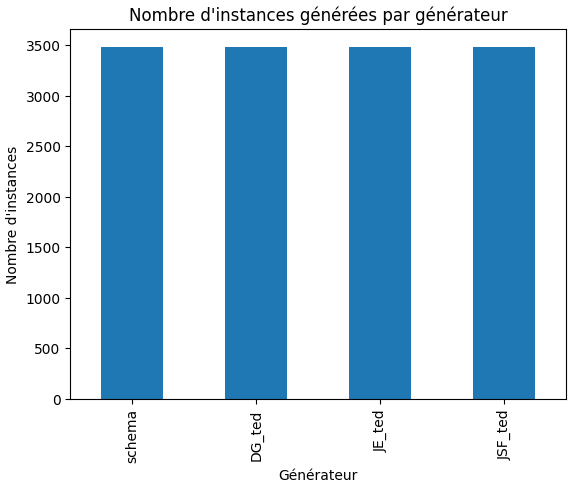
\includegraphics[scale=0.7]{Photos/ted_vs_errors/nb_instance_filtree.PNG}
      \caption{Nombre d'instance par générateur}
      \label{fig:nb_instance_filtree}
    \end{figure}
  \section{Génération d'instance Valide}
    La génération d'instances JSON Schema vise à créer des ensembles de données valides à partir d'un schéma JSON défini. Ce processus 
    est crucial pour divers cas d'utilisation, tels que la création de jeux de test, le remplissage de bases de données et l'exploration 
    de l'espace de solutions défini par le schéma \cite{GENERATION}. Pour celà on dispose des schémas, ainsi que des instances correctes, et nous utilisons trois générateurs d'instance, ces instances seront appelé witness : 
      \begin{itemize}
          \item [\textbullet] \textbf{json-schema-faker (JSF):} pour une génération rapide et simple de données fictives\cite{faker}.
          \item [\textbullet] \textbf{json-everything (JE):} écrite en C\#, est extension de \textbf{System.Text.Json}, limitée en termes d'expressivité sur la partie JSON\cite{everything}.
          \item [\textbullet] \textbf{json-data-generator (DG):} pour une prise en charge complète de JSON Schema Draft 7 et la génération de données aléatoires\cite{data_generator}.
      \end{itemize}

    
    Le dataset contenant les witness a été déjà construit précédemment, donc on mènera nos tests dessus
      
  \section{Distance d'édition et erreurs des instances}
    Une première approche serait de voir si il existe un lien entre la distance d'édition et le nombre d'erreurs pour chaque witness, celà en calculant la distance d'édition 
    entre chaque instance correct et les witness de chaque générateurs
      \subsection{Distribution des tailles}
        Pour cette partie on s'intéresse à la distribution des tailles des instances corrects ainsi que les witness. 
        \begin{figure}[H]
          \centering
          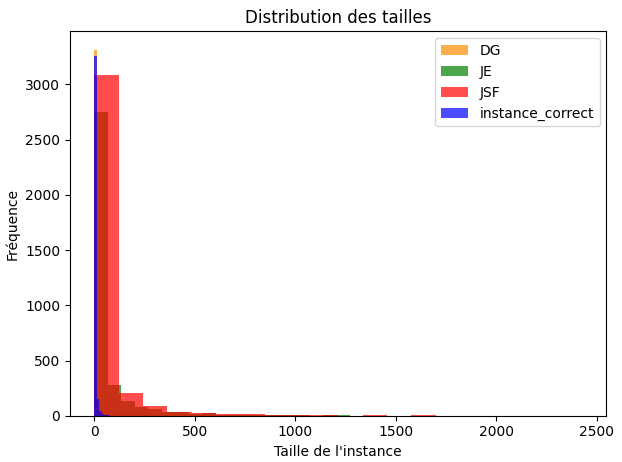
\includegraphics[scale=0.7]{Photos/ted_vs_errors/distribution_tailles.PNG}
        \end{figure}
      \subsection{Distribution des distances d'édition}
        On s'intéresse dans cette partie à savoir connaitre certaines statistiques concernant les distances d'édition pour chacun des générateurs 
        \begin{figure}[H]
          \begin{subfigure}[t]{\linewidth}
            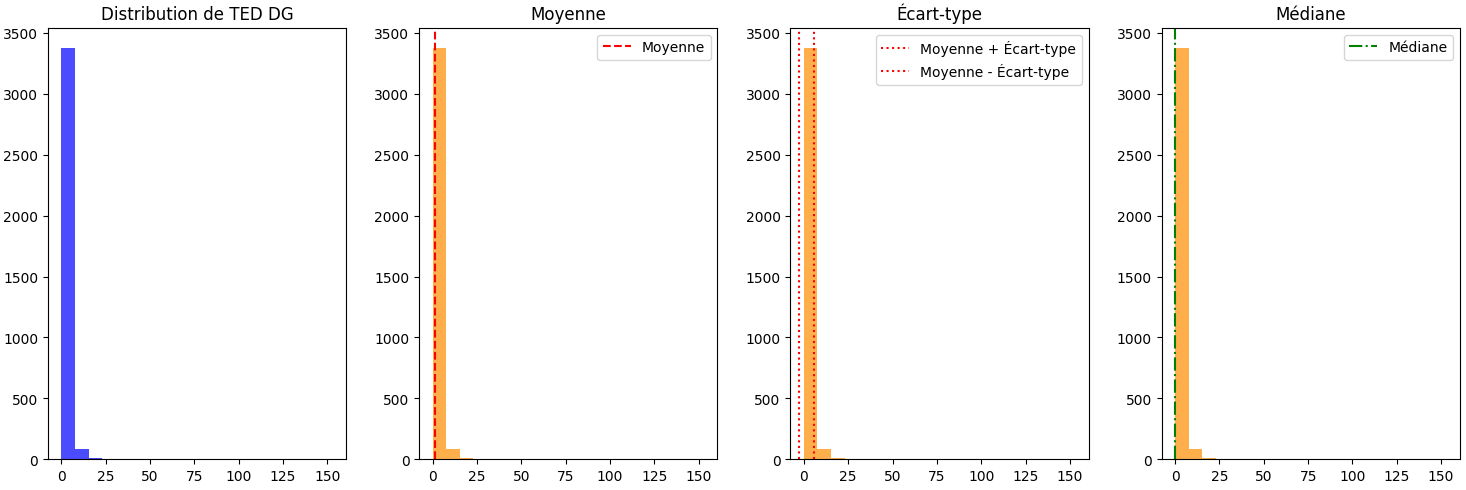
\includegraphics[scale=0.41]{Photos/ted_vs_errors/distribution_ted_dg.PNG}
            \caption{Distrubtion TED DG}
          \end{subfigure}
         
          \caption{Distribution des TED}
          \label{fig:distribution_ted}
        \end{figure}
        \begin{figure}[H]\ContinuedFloat
          \begin{subfigure}[t]{\linewidth}
            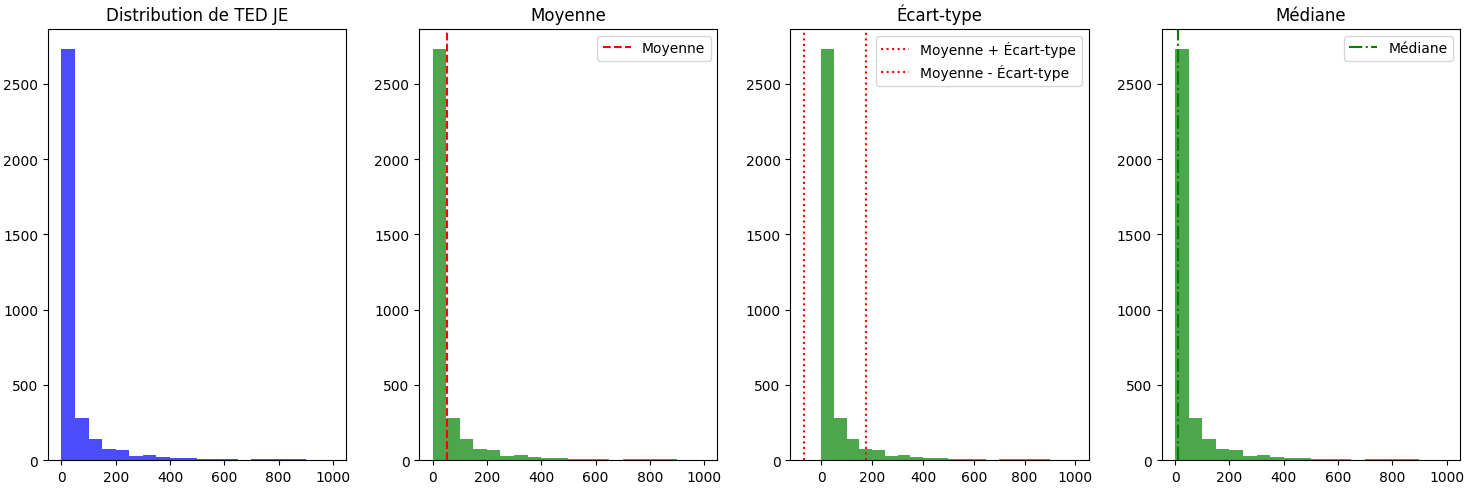
\includegraphics[scale=0.41]{Photos/ted_vs_errors/distribution_ted_je.PNG}
            \caption{Distrubtion TED JE} 
          \end{subfigure}
          \begin{subfigure}[t]{\linewidth}
            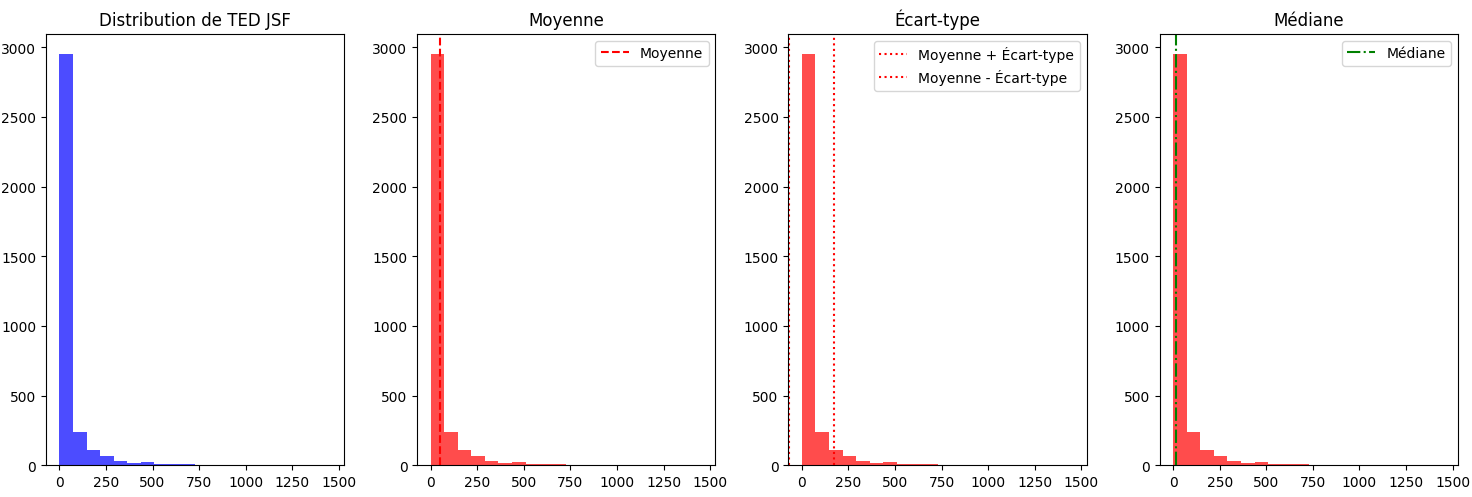
\includegraphics[scale=0.41]{Photos/ted_vs_errors/distribution_ted_jsf.PNG}
            \caption{Distrubtion TED JSF}
          \end{subfigure}
          \caption{Distribution des tailles des instances}
          \label{fig:distribution_tailles}
        \end{figure}

      
      \subsection{Relation entre distance d'édition et nombre d'erreurs}
        On s'intéresse dans cette partie à savoir connaitre certaines statistiques concernant les distances d'édition pour chacun des générateurs 
        \begin{figure}[H]
            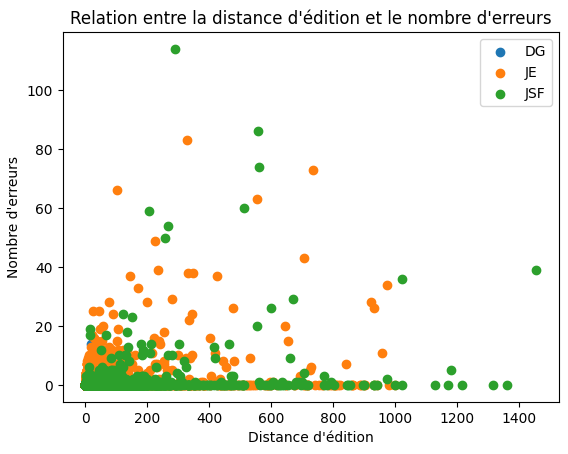
\includegraphics[scale=1]{Photos/ted_vs_errors/ted_vs_nb_errors.PNG}
            \caption{Nombre d'erreurs et TED }
          \label{fig:ted_vs_errors}
        \end{figure}

        On s'intéresse aussi à la relation entre la taille des witness par rapport à leurs TED (de l'instance correct) 
        \begin{figure}[H]
          \begin{subfigure}[t]{0.45\linewidth}
            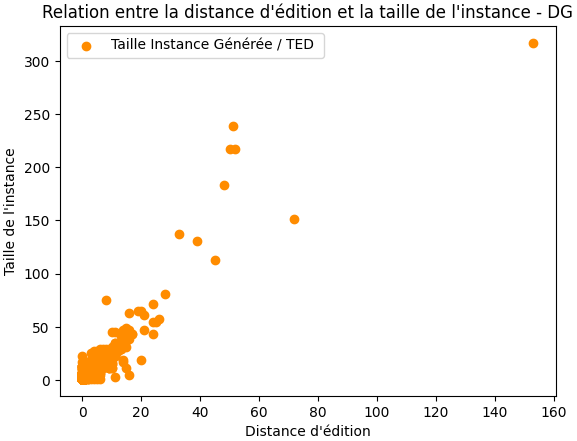
\includegraphics[scale=0.45]{Photos/ted_vs_errors/taille_vs_ted_dg.PNG}
            \caption{Taille d'instances et TED (DG)}
          \end{subfigure}
          \hfill
          \begin{subfigure}[t]{0.45\linewidth}
            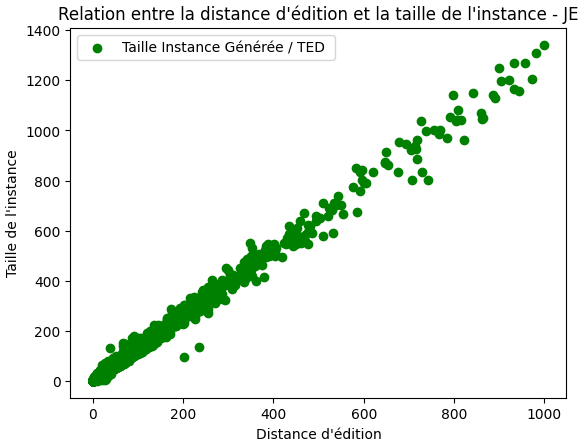
\includegraphics[scale=0.45]{Photos/ted_vs_errors/taille_vs_ted_je.PNG}
            \caption{Taille d'instances et TED (JE)}
          \end{subfigure}
          
          
          \caption{Distribution des TED}
          \label{fig:ted_vs_taille}
        \end{figure}
        \begin{figure}[H]\ContinuedFloat
          \centering
          \includegraphics[scale=0.5]{Photos/ted_vs_errors/taille_vs_ted_jSF.PNG}
          \caption{Taille d'instances et TED (JSF)}
        \end{figure}
      
      \subsection{Observations} 
        D'après notre étude expérimentale, nous observons qu'il n'existe pas de corrélation entre le nombre d'erreurs et la distance d'édition, 
        on remarque aussi que parfois la distance d'édition peut être assez grande et que le nombre d'erreurs ne soit pas si important ce résultat 
        est trivial car les instances génèrent des instances qui sont conforme au schéma mais qui ne sont pas une réplique de l'instance correct. On peut par contre 
        trouver une corrélation entre la taille des instances par rapport à la distance d'édition.
      \subsection{Conclusion}
        À ce niveau, la distance d'édition nous ne permet pas de déduire grande chose sur la réparation des instances, la raison principale est que JEDI nous donne qu'une mesure 
        quantitative sur le nombre d'opérations nécessaires, mais aucun information sur les opérations elles mêmes. 
        % Une des contraintes qu'on rencontre à ce niveau, c'est que JEDI ne garde aucune informations sur les opérations à faire sur 

